\documentclass{article}

\usepackage{graphicx}
\usepackage{tikz}
\usepackage{tikzsymbols}
\usetikzlibrary{calc,patterns,shapes.geometric}
\pagestyle{empty}
\usepackage[margin=0pt]{geometry}
\geometry{papersize={14in,12in}}

\def\centerarc[#1](#2)(#3:#4:#5){\draw[#1] ($(#2)+({#5*cos(#3)},{#5*sin(#3)})$) arc (#3:#4:#5);}

\begin{document}
	\begin{figure}
		\centering
		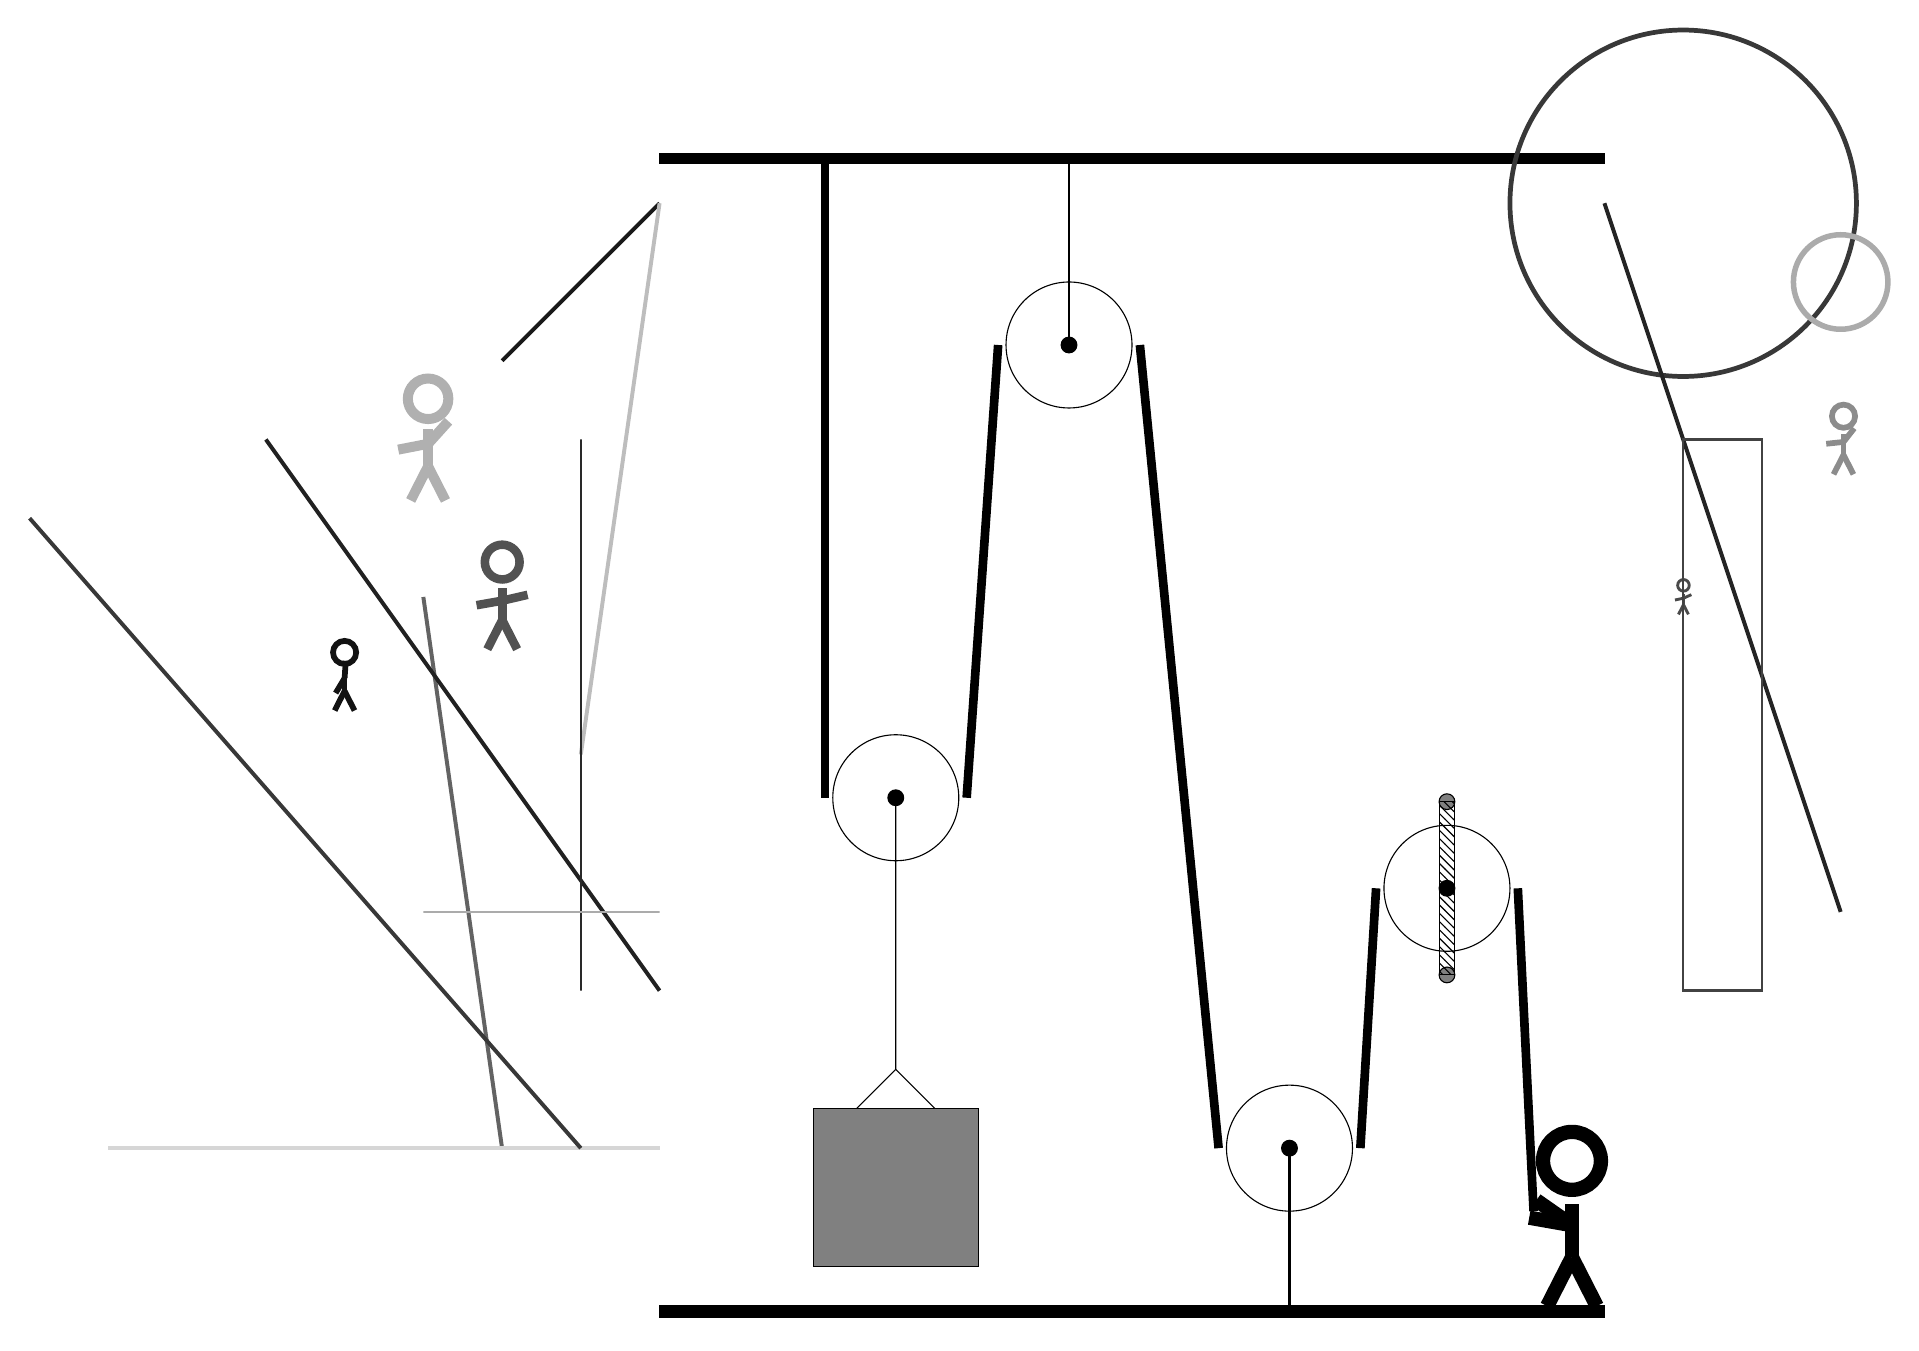
\begin{tikzpicture}
			%%%%% START %%%%%
			
			\draw[fill=black] (-2, 11.5) rectangle (10, 11.625);
			
			\draw (1, 3.45) circle (0.8);
			\draw[fill=black] (1, 3.45) circle (0.1);
			
			\draw (3.2, 9.2) circle (0.8);
			\draw[fill=black] (3.2, 9.2) circle (0.1);
			\draw[thick] (3.2, 9.2) -- (3.2, 11.5);
			
			\draw (6, -1) circle (0.8);
			\draw[fill=black] (6, -1) circle (0.1);
			\draw[thick] (6, -1) -- (6, -3);
			
			\draw[fill=white](8, 2.3) circle (0.8);
			\draw[fill=black] (8, 2.3) circle (0.1);
			\draw[fill=black!50] (8, 3.4) circle (0.1);
			\draw[fill=black!50] (8, 1.2) circle (0.1);
			\draw[pattern=north west lines, pattern color=black] (7.9, 3.4) rectangle (8.1, 1.2);
			
			\draw (1, 3.45) -- (1, 0.0) -- (0.5, -0.5);
			\draw (1, 0.0) -- (1.5, -0.5);
			\draw[fill=black!50] (-0.05, -0.5) rectangle (2.05, -2.5);
			
			\draw[line width=1.1mm] (0.1, 11.5) -- (0.1, 3.45);
			\centerarc[line width=1.1mm](1, 3.45)(180:360:0.9);
			\draw[line width=1.1mm](1.9, 3.45) -- (2.3, 9.2);
			\centerarc[line width=1.1mm](3.2, 9.2)(0:180:0.9);
			\draw[line width=1.1mm](4.1, 9.2) -- (5.1, -1);
			\centerarc[line width=1.1mm](6, -1)(180:360:0.9);
			\draw[line width=1.1mm](6.9, -1) -- (7.1, 2.3);
			\centerarc[line width=1.1mm](8, 2.3)(0:180:0.9);
			\draw[line width=1.1mm](8.9, 2.3) -- (9.1, -1.8);
			
			\node at (9.5, -1.9) {\Strichmaxerl[10][-35][170]};
			
			\draw [line width=0.6mm, color=black!78](11, 11) circle (2.2);
			
			\node[line width=0.6mm, color=black!68] at (-4, 6) {\Strichmaxerl[6][10][13]};
			\draw[line width=0.5mm, color=black!90](-2, 11) -- (-4, 9);
			\draw[line width=0.5mm, color=black!61](-5, 6) -- (-4, -1);
			\draw [line width=0.7mm, color=black!33](13, 10) circle (0.6);
			
			\node[line width=0.2mm, color=black!93] at (-6, 5) {\Strichmaxerl[4][59][86]};
			
			\node[line width=0.4mm, color=black!71] at (11, 6) {\Strichmaxerl[2][12][24]};
			\draw[line width=0.5mm, color=black!16](-2, -1) -- (-9, -1);
			\draw[line width=0.5mm, color=black!86](10, 11) -- (13, 2);
			\draw[line width=0.5mm, color=black!26](-3, 4) -- (-2, 11);
			\node[line width=0.4mm, color=black!45] at (13, 8) {\Strichmaxerl[4][6][52]};
			\draw[line width=0.3mm, color=black!74] (11, 1) rectangle (12, 8);
			\draw[line width=0.5mm, color=black!87](-7, 8) -- (-2, 1);
			
			\node[line width=0.6mm, color=black!31] at (-5, 8) {\Strichmaxerl[7][11][48]};
			\draw[line width=0.2mm, color=black!84] (-3, 8) rectangle (-3, 1);
			\draw[line width=0.3mm, color=black!33] (-2, 2) rectangle (-5, 2);
			
			\draw[line width=0.5mm, color=black!78](-3, -1) -- (-10, 7);
			
			\draw[fill=black] (-2, -3) rectangle (10, -3.15);
			
			%%%%% END %%%%%
		\end{tikzpicture}
	\end{figure}	
\end{document}